\chapter{Foundations}
\label{chap:foundations}

In this chapter topics that are tackled during the lecture are introduced in a basic fashion. This includes agents, sensor, actuators, communication, etc\dots

\section{Agents}
\label{sec:agents}

Although not every agent is autonomous, our focus in this lecture is to design autonomous agents. Autonomous means, that the agent is not controlled from some external entity. It only perceives its environment and acts in order to change it. Why it tries to change its environment depends on the agent's properties. Agents can be reactive or proactive, they can communicate with other agents, remember the history of the environment, and predict the future of the environment according to some model. As a designer of the agents, you need to decide what kind of agents you need to achieve your goal. The famous book \emph{Artificial Intelligence \textendash\ A Modern Approach}, written by Russel and Norvic, elaborates properties of agents and environment in chapter two. The book is available in our library. It is recommended to read chapter two for your exam preparations.

\subsection{Robot Control Architectures}
\label{ssec:robotcontrolarch}

\begin{figure}[htbp]
  \centering
  \begin{tikzpicture}[every node/.append style={thick}]
    \node(Agent)[plan, minimum width=2.5cm] at (0,0) {Agent};
    \node(Environment) [plan, minimum width=2.5cm] at (0,-1) {Environment};
    \draw[->, bend left] (Agent.south east) to node[right] {act} (Environment.north east);
    \draw[->, bend left] (Environment.north west) to node[left] {perceive} (Agent.south west);
  \end{tikzpicture}
  \caption{Simple Control Loop}
  \label{fig:simplecontrolloop}
\end{figure}

Usually it is believed that the agent is interacting with its environment \textendash whatever that environment is. This relation is often depicted as an agent-environment cycle (see Figure~\ref{fig:simplecontrolloop}). As mentioned before, the details of an agent architecture do vary from use case to use case.

\begin{figure}[htbp]
  \centering
  \begin{tikzpicture}[every node/.append style={thick}]

    \node(Data) at (0,0) {Data Layers};
    \node(SymbolLayer)[highLayer, anchor=north] at (Data.south) {};
    \node(SymbolLayerText)[anchor=north west] at (SymbolLayer.north west) {\tiny{\textbf{Symbol Layer}}};
    \node(SymbolLayerData)[data] at (SymbolLayer.south west) {\tiny{\textbf{Data:}\\[0.5em]Symbols, Rules,\\ Relations}};

    \node(IntermediateLayer)[midLayer, anchor=north west] at (SymbolLayer.south west) {};
    \node(IntermediateLayerText)[anchor=north west] at (IntermediateLayer.north west) {\tiny{\textbf{Intermediate Layer}}};
    \node(IntermediateLayerData)[data] at (IntermediateLayer.south west) {\tiny{\textbf{Data:}\\[0.5em]Feature Vectors, Raw Map}};

    \node(SensorimotorLayer)[lowLayer, anchor=north west] at (IntermediateLayer.south west) {};
    \node(SensorimotorLayerText)[anchor=north west] at (SensorimotorLayer.north west) {\tiny{\textbf{Sensorimotor Layer}}};
    \node(SensorimotorLayerData)[data] at (SensorimotorLayer.south west) {\tiny{\textbf{Data:}\\[0.5em]Raw Data}};

    \node(ButtomUp)[single arrow, shape border rotate=90, draw, anchor=center, minimum height=5.02cm, xshift=-1cm, text width=1cm, align=center] at (IntermediateLayer.west) {\tiny{Data Abstraction}};
    \draw[->, bend right] (IntermediateLayerData.east) to node [processingArrow] {\tiny{Symbol\\Grounding,\\Anchoring}} (SymbolLayerData.south east);
    \draw[->, bend right] (SensorimotorLayerData.east) to node [processingArrow] {\tiny{Smoothing,\\ Filtering}} (IntermediateLayerData.south east);

    \node(Processing) at (6,0) {Control Layers};
    \node(DeliberateLayer)[highLayer, anchor=north] at (Processing.south) {};
    \node(DeliberateLayerText)[anchor=north west] at (DeliberateLayer.north west) {\tiny{\textbf{Deliberation Layer}}};
    \node(DeliberateLayerData)[data] at (DeliberateLayer.south west) {\tiny{\textbf{Control:}\\[0.5em]Communication, Planning, Strategy Evaluation}};

    \node(SequencerLayer)[midLayer, anchor=north west] at (DeliberateLayer.south west) {};
    \node(SequencerLayerText)[anchor=north west] at (SequencerLayer.north west) {\tiny{\textbf{Sequencer Layer}}};
    \node(SequencerLayerData)[data] at (SequencerLayer.south west) {\tiny{\textbf{Control:}\\[0.5em]Path Planning, Strategy}};

    \node(ControlLayer)[lowLayer, anchor=north west] at (SequencerLayer.south west) {};
    \node(ControlLayerText)[anchor=north west] at (ControlLayer.north west) {\tiny\textbf{{Reactive Control Layer}}};
    \node(ControlLayerData)[data] at (ControlLayer.south west) {\tiny{\textbf{Control:}\\[0.5em]Reaction,\\Controlling}};

    \node(TopDown)[single arrow, shape border rotate=270, draw, anchor=center, minimum height=5.02cm, xshift=+1cm, text width=1cm, align=center] at (SequencerLayer.east) {\tiny{Decision Making and Execution}};
    \draw[<-, bend left] (SequencerLayerData.west) to node [processingArrow, text width=1cm, left, yshift=2mm] {\tiny{Strategy\\Adaption}} (DeliberateLayerData.south west);
    \draw[<-, bend left] (ControlLayerData.west) to node [processingArrow, text width=1.1cm, left, yshift=2mm] {\tiny{Behaviour\\Adaption}} (SequencerLayerData.south west);

    \node(Environment) [minimum width=9cm, minimum height=0.8cm, draw=black!85] at (3,-7) {Environment};
    \draw[->, bend right] (ControlLayerData.west) to node [left] {\tiny{act}} ([xshift=1.3cm]Environment.north);
    \draw[->, bend right] ([xshift=-1.8cm]Environment.north) to node [right] {\tiny{sense}} (SensorimotorLayerData.east);

    \draw[<->] ([yshift=5mm]SymbolLayer.east) to ([yshift=5mm]DeliberateLayer.west);
    \draw[<->] ([yshift=-5mm]IntermediateLayer.east) to ([yshift=-5mm]SequencerLayer.west);
    \draw[<->] (SensorimotorLayer.east) to (ControlLayer.west);
  \end{tikzpicture}
  \caption{Control Loop}
  \label{fig:controlloop}
\end{figure}

In Figure~\ref{fig:controlloop} an overview of the details of a state-of-the-art robot control system is shown. You should consider a robot as a physical agent, i.d., an agent with a physical representation. The Data Layers on the left hand side represent the utilised algorithms to gain information and knowledge from raw sensor data. During the data processing, the data is continuously filtered, condensed, and abstracted until symbols and relations can be integrated into a symbolic knowledge representation. This knowledge is required by the algorithms on the right hand side of Figure~\ref{fig:controlloop}. The Deliberation Layer, including algorithms for planning, communication, and strategy evaluation, computes its decisions based on the knowledge of the symbolic knowledge representation. The results are processed by the Sequencer Layer and transformed into commands for controlling actuators of the robot.

The data abstraction and decision making cycle is not perfectly followed in all applications. Often the abstraction of data up to the level of symbols and relations is not necessary. Moreover, it isn't clever to make everything a decision on the top most available layers. Think of a robot control architecture as of a human brain. A lot of things in a human body are handled without having the brain actively thinking about it, e.g., breathing, heart beat, reflexes on your knee, sneezing, blinking, etc. For a robot the corresponding things could be obstacle avoidance, motor controlling, avoiding rough terrain such as stairs, etc. Things like that should also in a robot control architecture be handled on lower levels and not bothering algorithms for planning or communication.

However, don't take this easy. It can be quit difficult or even impossible to assign a certain task to a certain level. Obstacle avoidance, for example, is sometimes part of all three layers: While driving along a path, the robot in a office environment avoids humans or other robots by directly reacting to its 2D distance scans from its laser scanner (lower layers). The path itself is planned in order to avoid already known walls and finding the shortest path (intermediate layers). Planning this path is influenced by some knowledge about the environment, e.g., the robot knows that there is currently a meeting going on in some room and as the robots motion is relative noisy, it knows that it should avoid meetings like a virtual obstacle, in order to not disturb the meeting (top layers).

If you are in the position to decide on which layer something should be implemented, it sometimes helps to think about the following. The effort for abstracting data rises with each necessary processing step, therefore creating symbolic knowledge is often very costly. On the one hand, this argues for putting everything as on the lowest levels. On the other hand, the data on the lowest levels is often very large in terms of memory. You often have to ponder, whether it is more efficient to abstract the data and thereby reduce it to the smallest possible size or whether it is more efficient to directly operate on millions of raw camera pixel values without explicitly representing objects in the environment. Sometimes technical limitations also force you to a certain direction. If your robots, for example, need to communicate about objects it is probably impossible to send whole images of the objects to each other due to bandwidth limitations. Instead, the objects have to be abstracted to symbols or coordinates in order to match the bandwidth restrictions.

\section{Sensors}
\label{sec:sensor}

Sensors are the only option for an agent to perceive its environment. This also means, that everything that helps an agent to perceive its environment can be considered as a sensor. Nevertheless, sensors are also used to measure internal values, not belonging to the environment. Before we are going to deep, let us start the sensor topic a little bit more general.

\subsection{Sensor Categories}
\label{ssec:sensorcategories}

There are two sensor properties that help to categorise the plethora of sensors available nowadays: Active vs. passive sensors and external vs. internal sensors. Whether a sensor is active or passive determines the way it measures some value.

\begin{description}
 \item [active:] An active sensor emits something, e.g., energy, for measuring what ever it should measure. Typical examples are laser scanners or radars that emit electro-magnetic waves of different wave length.
 \item [passive:] Passive sensors directly measure energy from the environment. A camera for example perceives sunlight that is reflected from a surface, furthermore a compass measures the terrestrial magnetic field.
\end{description}

The difference between an internal or external sensor are the type of values the sensor measures, not how it measures it.

\begin{description}
 \item [internal:] Internal sensors measure values that are part of the system itself. Therefore it depends on the borders between the system and its environment. In case of a robot an internal sensor value could be its battery levels.
 \item [external:] External sensors measure values from the outside of the system, i.d., values from its environment. Typical values are distances, light, and sound.
\end{description}

\subsection{Sensor Properties}
\label{ssec:sensorproperties}

Subsection~\ref{ssec:sensorcategories} is for categorising different types of sensors. If you need to choose a sensor for your application these categories are only a first orientation. In this subsection you will get a short overview of general things you have to consider in your decision for taking the right sensor for your application.

\begin{description}
 \item [Size] Does the sensor fit into your robot?
 \item [Weight] Can the sensor be lifted or carried by your robot (especially relevant for drones)?
 \item [Energy Consumption] Does the energy consumption of the sensor significantly reduce the runtime of your robot?
 \item [Sensor Range] Sensors often have minimum and maximum values they can measure, e.g., distance starting from 0.4m up to 100m. Does the range fit your application?
 \item [Field of View] In which direction can the sensor measure? Is it big enough? Can it be integrated into your robot without limiting the field of view?
 \item [Operating Conditions] Some sensors are sensitive to temperature, vibration, light and so on. Does your application match their operating conditions?
 \item [Resolution] What is the granularity of the measured values (directly influences properties from Subsection~\ref{ssec:valuepropoerties})?
 \item [Value Transformation] Is the value received from the sensor in the unit you need? If not, do you know the transformation and how long does the transformation take?
 \item [Linearity] Does a linear change in the value to be measured induce a linear change in the value received from the sensor? If not, what is the relation (see Value Transformation)?
\end{description}

\subsection{Sensor Value Properties}
\label{ssec:valuepropoerties}

The sensor value properties of possible sensors are very important for making the right choice, too. In this subsection we collect these properties, explain their meaning, and explain why they are important.

The sketched definitions given below follow the \href{https://en.wikipedia.org/wiki/Accuracy_and_precision#ISO_definition_.28ISO_5725.29}{ISO Standard 5725}.

\begin{description}
 \item [Precision] Precision is about the reproducability or repeatability of measurements. The sensor has a high precision, if it always measures the same values under same conditions. Note that this measured values can be completely wrong!
 \item [Accuracy] Accuracy is the average difference between the reference value (correct value) and the measured values. Please read this carefully, as it only slightly differs from trueness.
 \item [Trueness] Trueness is the difference between the reference value (correct value) and the average of the measured values.
\end{description}

\begin{figure}[htbp]
 \centering
 \begin{subfigure}[b]{0.5\textwidth}
 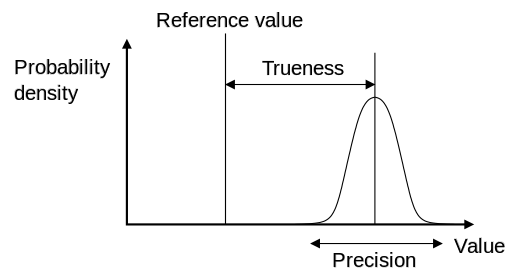
\includegraphics[width=\textwidth]{pic/trueness_and_precision.png}
 \caption{Trueness vs. Precision}
 \label{sfig:trueness_vs_precision}
 \end{subfigure}
 \begin{subfigure}[b]{0.2\textwidth}
 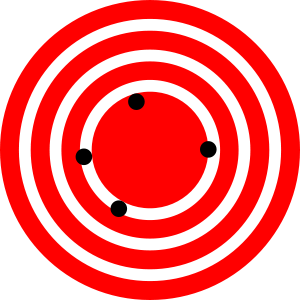
\includegraphics[width=\textwidth]{pic/High_accuracy_Low_precision.png}
 \caption{Low accuracy, poor precision, good trueness}
 \label{sfig:poor_precision}
 \end{subfigure}
 \begin{subfigure}[b]{0.2\textwidth}
 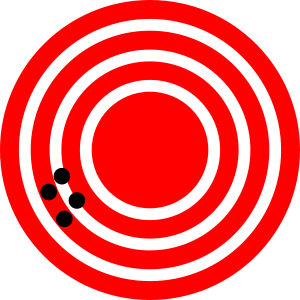
\includegraphics[width=\textwidth]{pic/High_precision_Low_accuracy.png}
 \caption{Low accuracy, good precision, poor trueness}
 \label{sfig:high_precision}
 \end{subfigure}
 \caption{Examples for Precision, Accuracy and Trueness (Source: \href{https://en.wikipedia.org/wiki/Accuracy_and_precision}{Wikipedia})}
 \label{fig:prec_accur_truen}
\end{figure}

In Figure~\ref{fig:prec_accur_truen} several helpful pictures for understanding the above definitions are given. Especially the targets make the difference between accuracy and trueness comprehensible. In order to get a feeling for the relevance of precision, accuracy and trueness in practice let us exercise the utilisation of sensors with different properties. Imaging your task is to get to know what the correct value for a certain distance is.

The easiest case is when you have a highly accurate sensor, because this means that each measurement is relatively close to the correct value. It also means that the precision of the sensor must be relatively high, too. Here is why: If all measurements are close to a single static value (being accurate), the measurements cannot vary very much at the same time (low precision).

Now let us consider to use a sensor with low accuracy, but with high precision (like in Subfigure~\ref{sfig:high_precision}). The measured values are relatively wrong, but the are reproduceable. Therefore, the sensor will measure under the same conditions the same wrong values. That gives you the chance to correct this relative constant offset or error by calibrating your sensor. For calibration you need a series of measurements for that you know the correct value. As you have a precise sensor, the difference between the measured values and the correct value should be more or less the same. In a naive calibration you could simply take this difference and correct the sensor's measurements by this difference at runtime. The problem is that precision means reproducability under the \textbf{same conditions}. These conditions often include the following parameters: the correct value, the state of the sensor (temperature, power supply, operation modes), and properties relevant for the measurement process (temperature, surfaces, light conditions). Therefore, calibration means to find the correct offset for all possible parameter combinations that influence the operating conditions of the sensor. Maybe this sounds like an almost unmanageable task, but here are some arguments against it:

\begin{itemize}
 \item The sensor already can calibrate itself with a special operation mode that you only have to trigger from time to time.
 \item The most parameters are irrelevant for the measuring.
 \item Have a look at your application scenario, hopefully a lot of parameters are constant in you application (artificial lights, indoor temperatures).
\end{itemize}

As a last relevant case, let us consider a sensor with low accuracy, but with high trueness (like in Subfigure~\ref{sfig:poor_precision}). Here the average of the measured values is relatively close the correct value. Therefore, you only need to take the average of some measurements, in order to know the correct value. The only question is: ``How much measurements are necessary?'' Simply make some experiments where you observe the change of the average relative to the increasing number of measurements. When the change of the average is low enough for your application you know the minimal number of measurements necessary to calculate a good average for determining the correct value. Think about your application then: Is it possible to make this number of measurements before the correct value changes, e.g., distance to moving obstacles. Obviously, you need more measurements if the standard deviation of the measurements is high, and less if its low. Note that a sensor with high trueness and a small standard deviation is actually an accurate sensor.

To summarise: Accurate sensors are fine, precise sensors need to be calibrated, and sensors with high trueness demand for calculating the average of some measurements.

\section{Actuators}
\label{sec:actuators}

Actuators are the counterpart to sensors. While an agent perceives its environment with the help of sensors, it changes its environment with the help of actuators. Let's consider some examples and try to derive general categories from it (see Figure~\ref{fig:actuator_examples}.

\begin{figure}[htbp]
 \begin{subfigure}[b]{0.3\textwidth}
  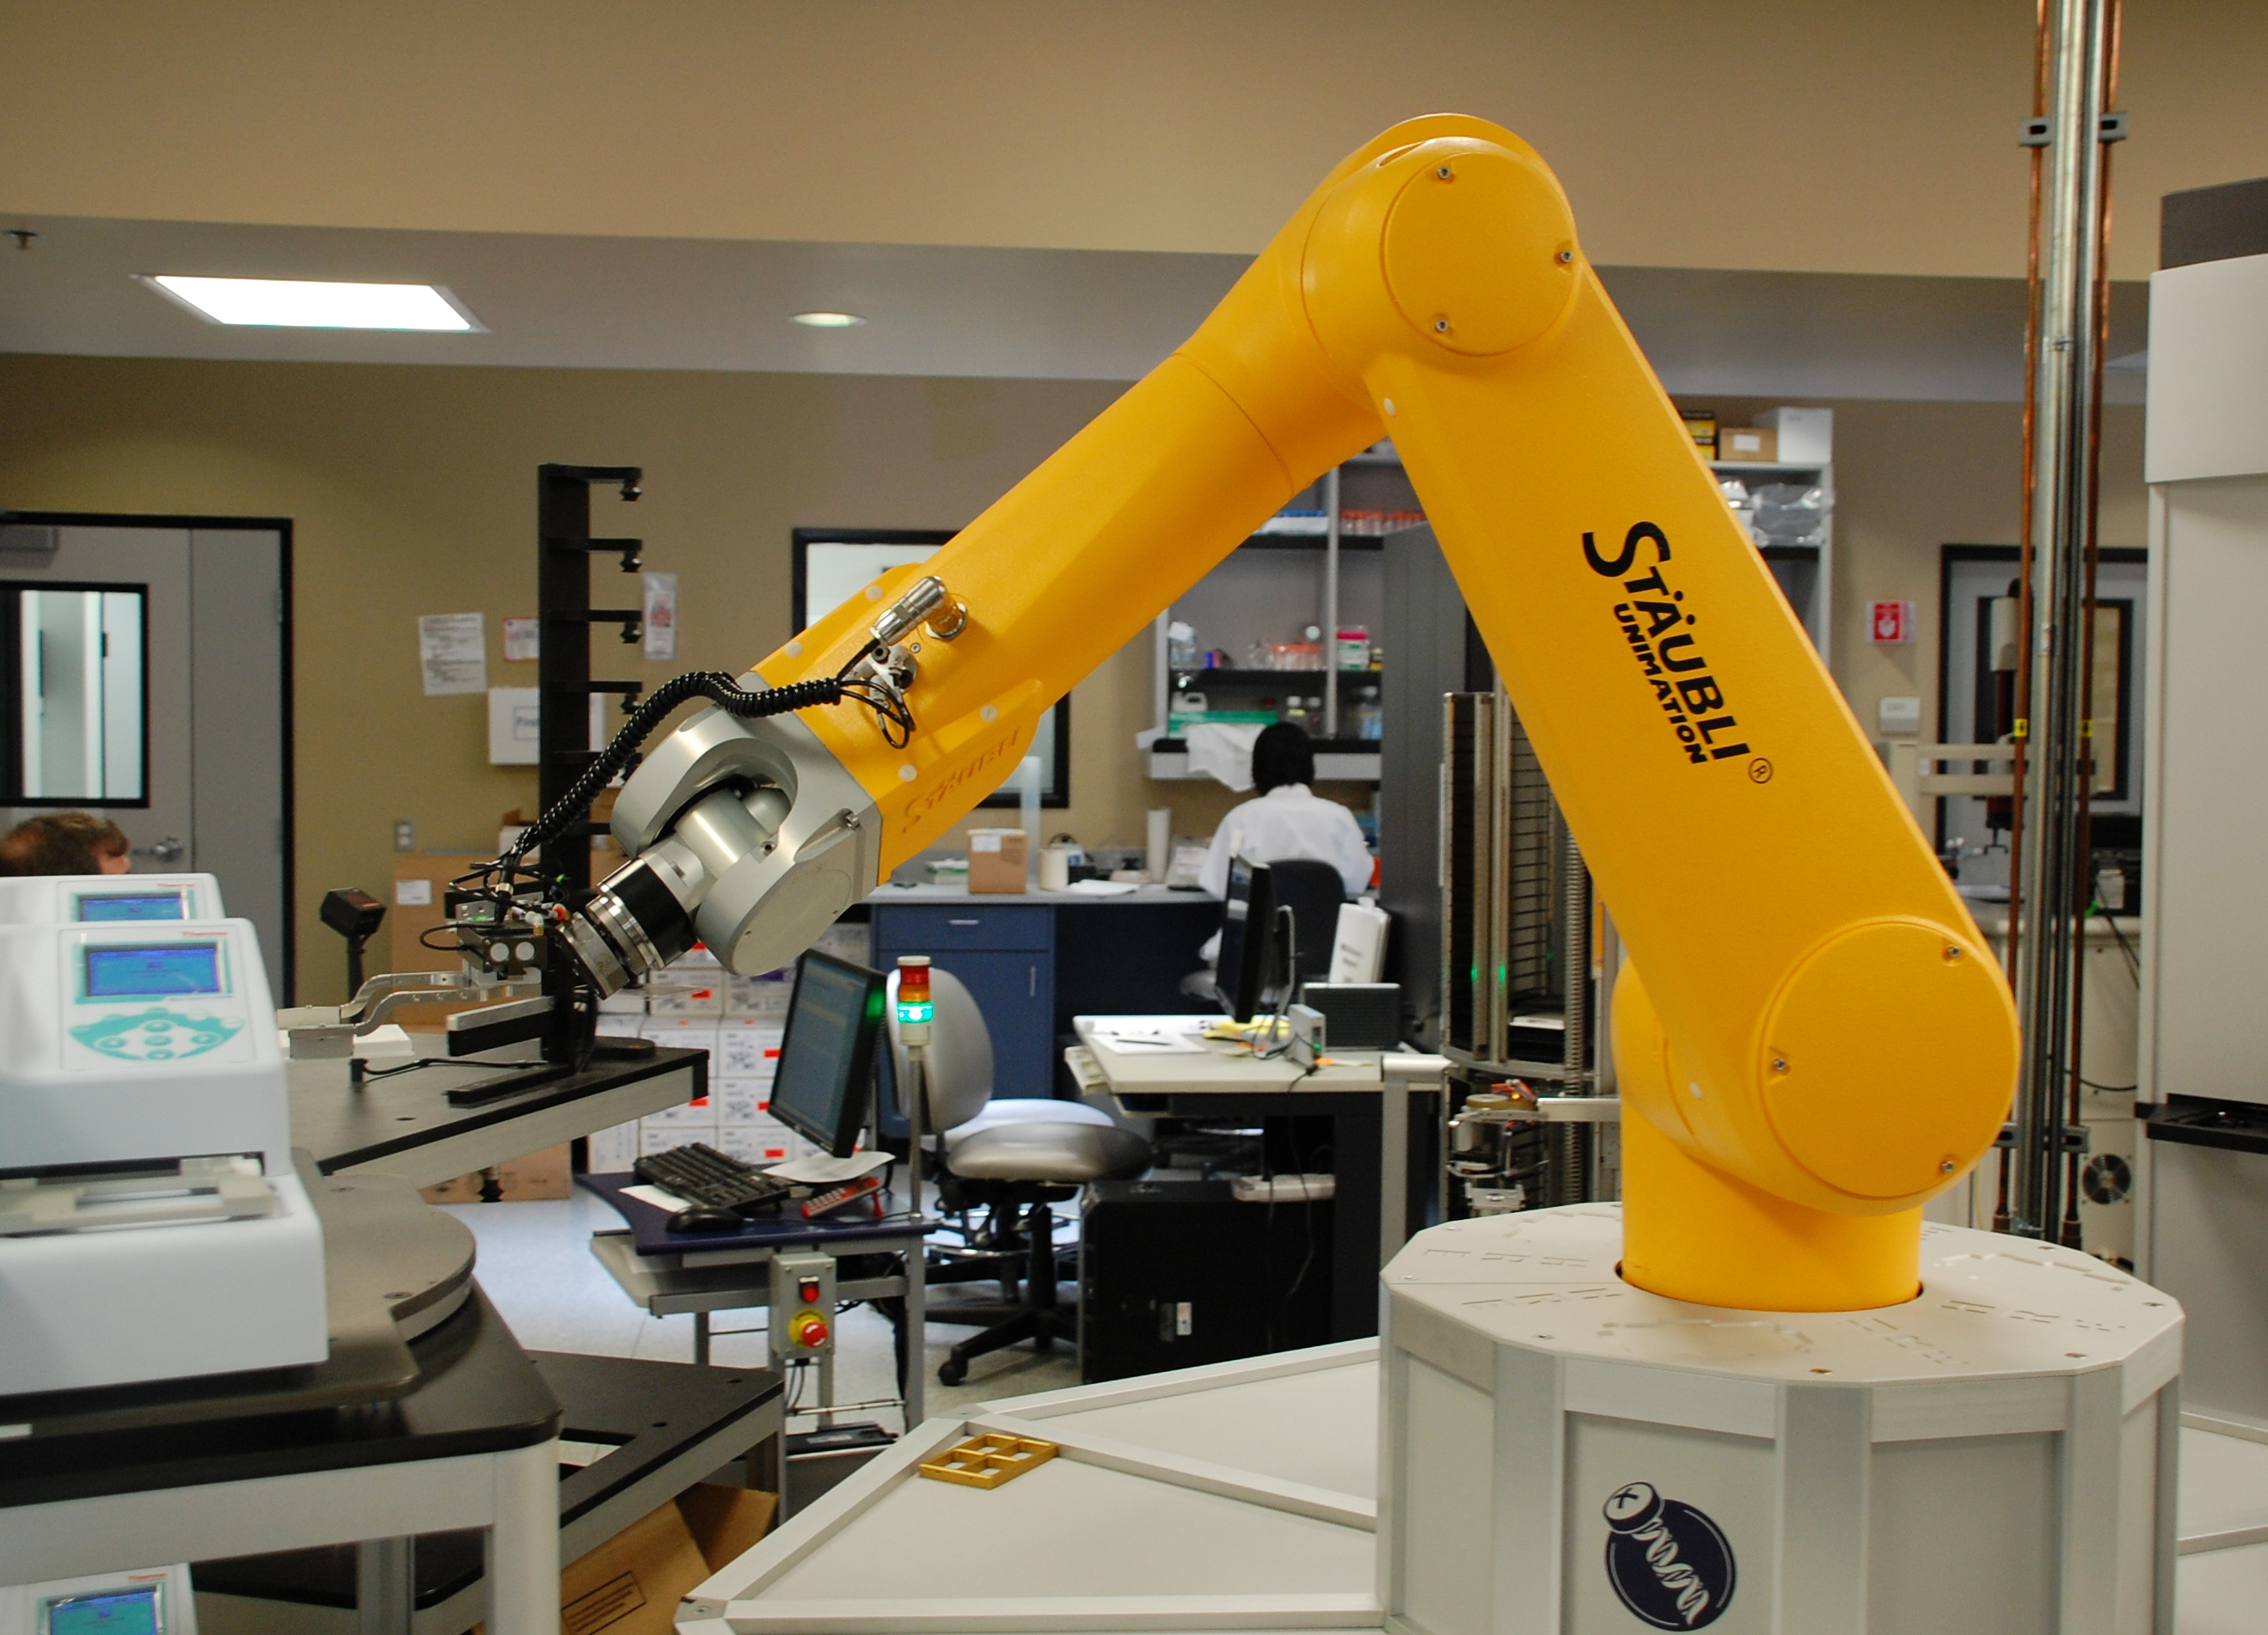
\includegraphics[height=3cm]{pic/RobotArm.jpg}
  \caption{Robot Arm (Source: \href{https://en.wikipedia.org/wiki/File:CPCCG_screening_robot.jpg}{Wikipedia})}
  \label{sfig:robot_arm}
 \end{subfigure}
 \quad
 \begin{subfigure}[b]{0.3\textwidth}
  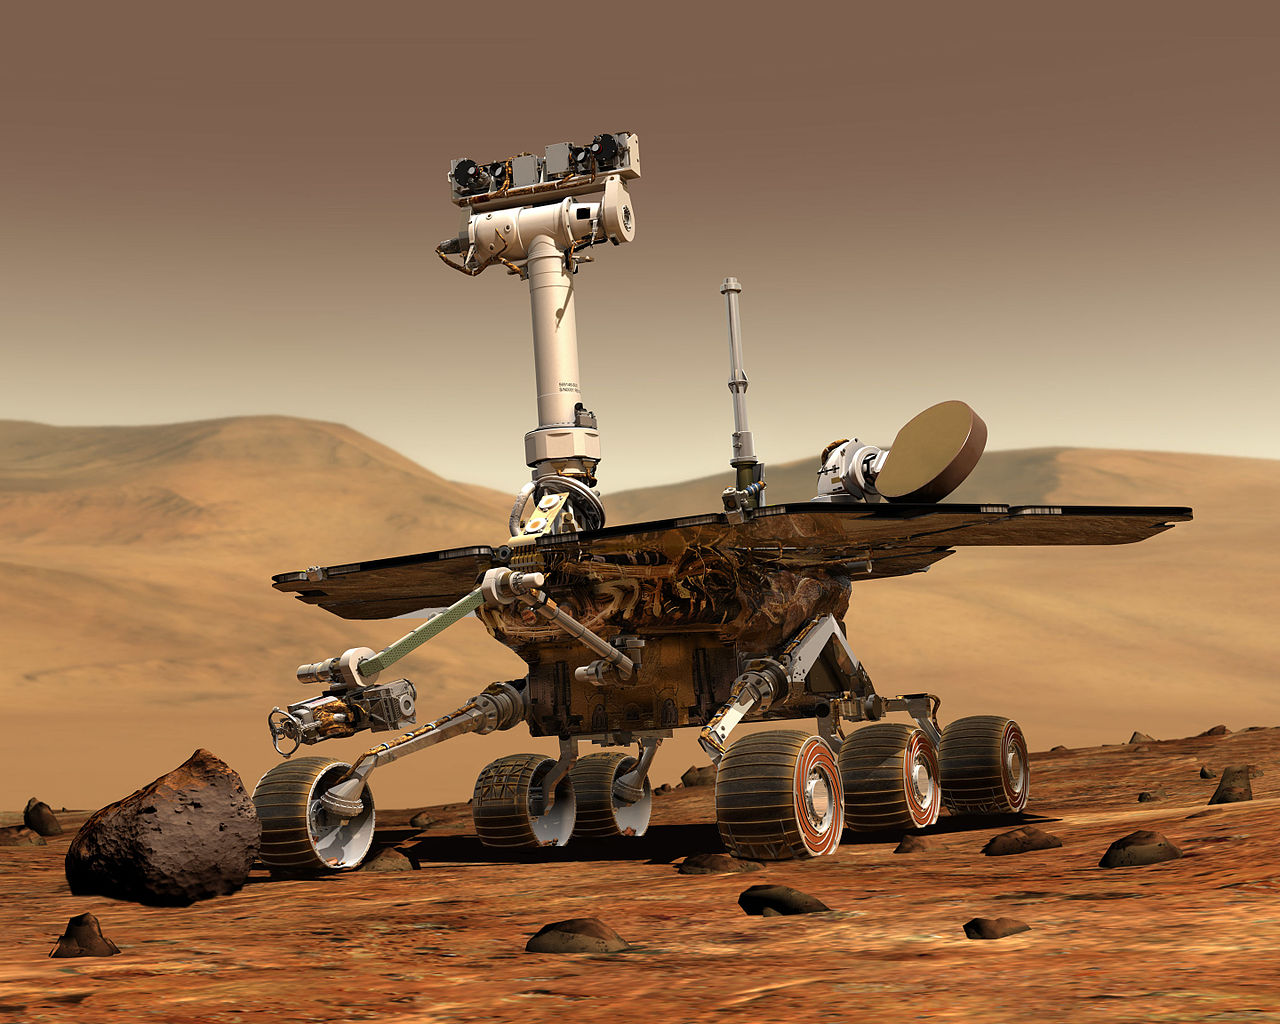
\includegraphics[height=3cm]{pic/RobotLocomotion.jpg}
  \caption{Robot Locomotion (Source: \href{https://en.wikipedia.org/wiki/Mars_Exploration_Rover\#/media/File:NASA_Mars_Rover.jpg}{Wikipedia})}
  \label{sfig:robot_locomotion}
 \end{subfigure}
 \quad
 \begin{subfigure}[b]{0.3\textwidth}
  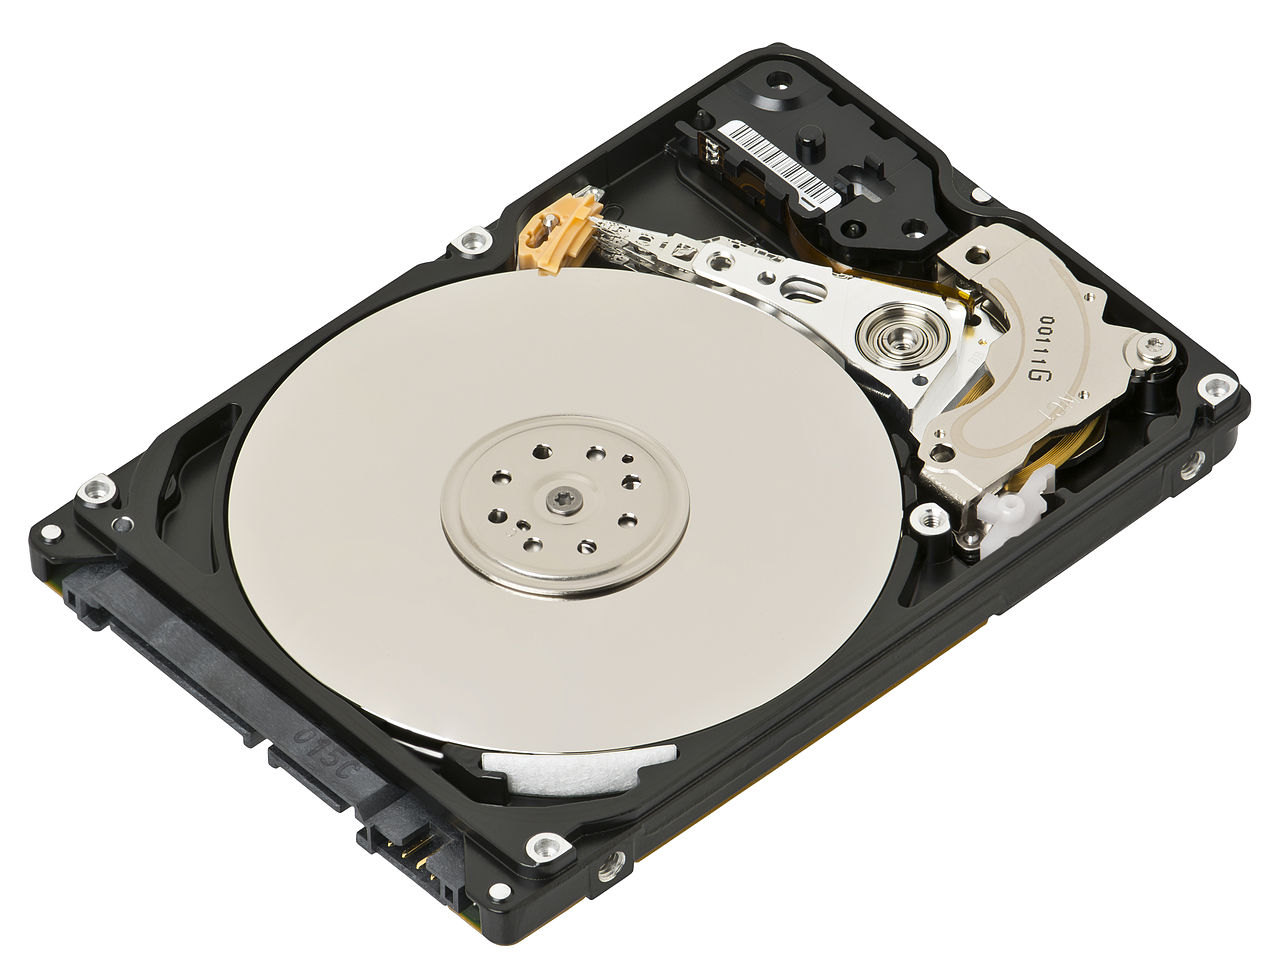
\includegraphics[height=3cm]{pic/HDD.jpg}
  \caption{Hard Disk Drive (Source: \href{https://en.wikipedia.org/wiki/Hard_disk_drive\#/media/File:Laptop-hard-drive-exposed.jpg}{Wikipedia})}
  \label{sfig:robot_locomotion}
 \end{subfigure}
 \caption{Examples for Actuators of Agents}
 \label{fig:actuator_examples}
\end{figure}

Subfigure~\ref{sfig:robot_arm} shows a robto arm in a laboratory environment. This arm can manipulate the environment, e.g., by executing pick-and-place tasks, but it also represents the whole robot. In the context of this lecture we barely consider this arm as a physical agent for the following reasons: It is not autonomous, it has no external sensors for perceiving its environment, and it probably does the same movements over and over again. However, imagine that this arm is mounted on a mobile platform and controlled by an autonomous control architecture (see Subsection~\ref{ssec:robotcontrolarch}) that is also able to perceive its environment through dedicated sensors. Let us collect a list of rather blunt and naiv statements about this actuator. 
\begin{itemize}
 \item The arm is made for manipulating the environment, so it is not just an actuator, it is a manipulator.
 \item It has a certain flexibility which is often denoted as degrees-of-freedom (DOF). 
 \item Reaching out from its mobile platform, its range is limited.
 \item Depending on its motors and energy sources, it can execute its movement with a limited force / speed.
 \item Depending on the mechanism at the end of the arm, it can only manipulate objects that suit this mechanism (denoted as Endeffector).
\end{itemize}



\section{Communication}
\label{sec:communication}
